\section{Evaluation}
\label{sec:evaluation}
This section presents a set of evaluations to show the performance of dynamic solution compared with the original ingress controller. We establish a kubernetes cluster to be the base of the whole evaluation. Then we emulate five workload patterns and run them for twice, one with the original ingress controller equiped, the other with our modified ingress controller equiped to compare their performance.
In summary, our results show that the modified ingress controller achieves better performance in most web cases. For
independent web applications, the modified ingress controller can balance load well even when there is a great difference between resource consumption of requests. Furthermore, in scaling case, modified ingress controller succeeds to split more load to the new idle endpoints, helping reduce pressure of high-load endpoints and improving RPS. For dependent web applications, modified ingress controller helps protecting endpoints from being influenced by node load, resource race against other endpoints and dependencies to other applications. Modified ingress controller addresses these cases with extra 1/3 overhead. The original ingress controller consumes about 32~35 millicore to synchronize endpoints changes while modified ingress controller consumes 10 more millicore for load monitor and dynamic load balancing.

\subsection{Configuration}

Our evaluate platform consist of a tsung server, a original ingress controller, our modified ingress controller, several test applications and datebases.
All these are deployed as pods on kubernetes. Our kubernetes cluster is made up of a master and five nodes. The hardware configuration of master is Intel Core processor i7 6700 with 4 CPU cores(3.4Ghz), 64GB system memory and
a 1TB HDD disk. Nodes share the same configuration: Intel Xeon processor E5 2620 with 8 cores (2.10Ghz), 64GB system memory and a 1TB HDD disk. Many system components are deployed on the master, because it is responsible for managing the whole cluster, making it in high-load state, so we do not put any workload on master.
The tsung server is a request generator to emulate workload pattern for comparing performance, and we deploy it alone on node1 without putting any other application on node1 to make sure its perfomance on generating requests is not influenced by other unrelated factors during the evaluation.
Similarly, to gurantee the pure performance, we let ingress controller deployed alone on node2. The test application is a java web application connected to a database, it has several apis exposed, requests of different api have diverse consumption on CPU,memory,network and database.
The database is a MySQL instance accessed by the test applications. We deploy test applications on node3, node4, node5 and database on node6. With different strategies to generate workload, different number and placement of test application and database, we emulate fix workload pattern to
compare performance.

\subsection{Workload Pattern}
\label{subsec:workload_pattern}
In this section, we evaluate four workload patterns to evaluate performance of modified ingress controller compared with original ingress controller.
The workload patterns include initialization pattern, scaling pattern, node-blocking pattern and database-blocking pattern with four different setting of
endpoint placement, scaling strategies and workload composition.
\begin{figure}[!htb]
 \centering
 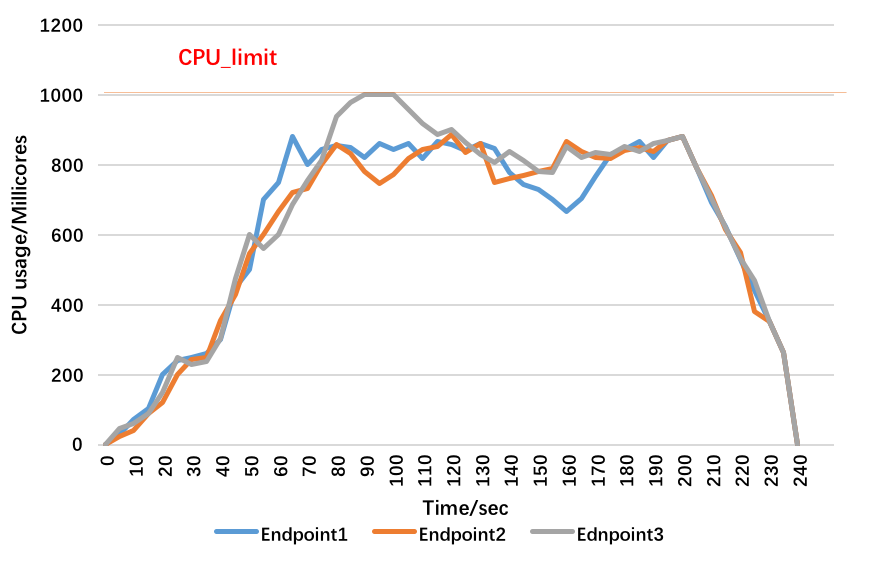
\includegraphics[width=0.45\textwidth]{images/data1.png}\\
 \caption{original controller under initialization pattern}
 \label{fig:original_initialization}
\end{figure}

\begin{figure}[!htb]
 \centering
 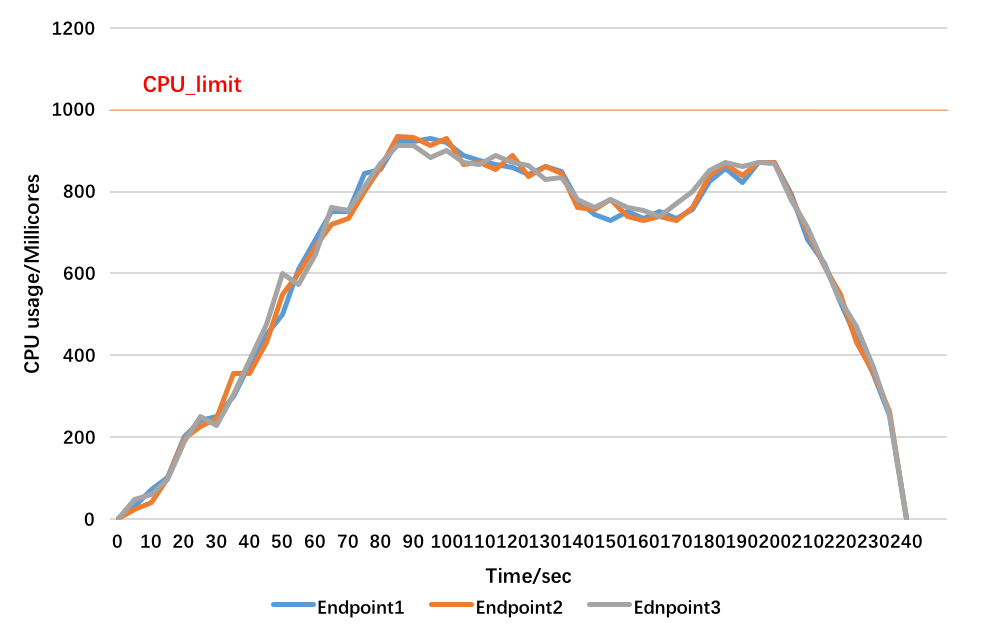
\includegraphics[width=0.45\textwidth]{images/data2.png}\\
 \caption{modified controller under initialization pattern}
 \label{fig:modified_initialization}
\end{figure}

Initialization pattern stands for the initial state when test applications are just deployed: we first deploy three replicas of test application, that is endpoint1 in node3, endpoint2 in node4 and endpoint3 in node5 to prevent that they are impacted by each other. After the deployment, we generate requests of all kinds at a fixed speed by tsung server to access test applications through ingress controller. For convenience, we use the cpu statistics to present performance. Figure~\ref{fig:original_initialization} presents the performance of original ingress controller under initialization pattern and figure~{\ref{fig:modified_initialization}} shows the performance of modified ingress controller. Result shows that for the original controller, load of endpoints become unstable and endpoint3 once becomes overhead(its cpu usage excceed its cpu limit) during 80s-100s, causing several requests return 503 to tsung server, it confirms that the default round-robin algorithm only performs well when resource consumption of requests are almost the same, which does not match the real circumstance initialization pattern describes: different kinds of requests have diverse resource requirements, under this circumstance, if we dispatch requests evenly to endpoints, some endpoints can become overhead presumably. Therefore, 503-request appears in evaluation for original ingress controller. Figure~{\ref{fig:modified_initialization}} shows that with the effort of modified ingress controller, there is no more overhead endpoint, load of endpoints are more even instead. More and more, table~{\ref{table:request_summary1}} points out that original ingress controller finishes 8892 reqeust, with 1108 503-requests, the modified ingress controller finishes 10000 requests with no 503-request, and the total number of requests is 10000.
\hspace{0pt}
\begin{table}[htbp]
 \begin{center}
  \begin{tabular}{c|c|c|c}
   \hline
            & Finished & 503  & Total \\  \hline
   Original & 8892     & 1102 & 10000 \\ \hline
   Modified & 10000    & 0    & 10000 \\ \hline
  \end{tabular}
 \end{center}
 \caption{Request summary of initialization pattern}
 \label{table:request_summary1}
\end{table}


\begin{figure}[!htb]
 \centering
 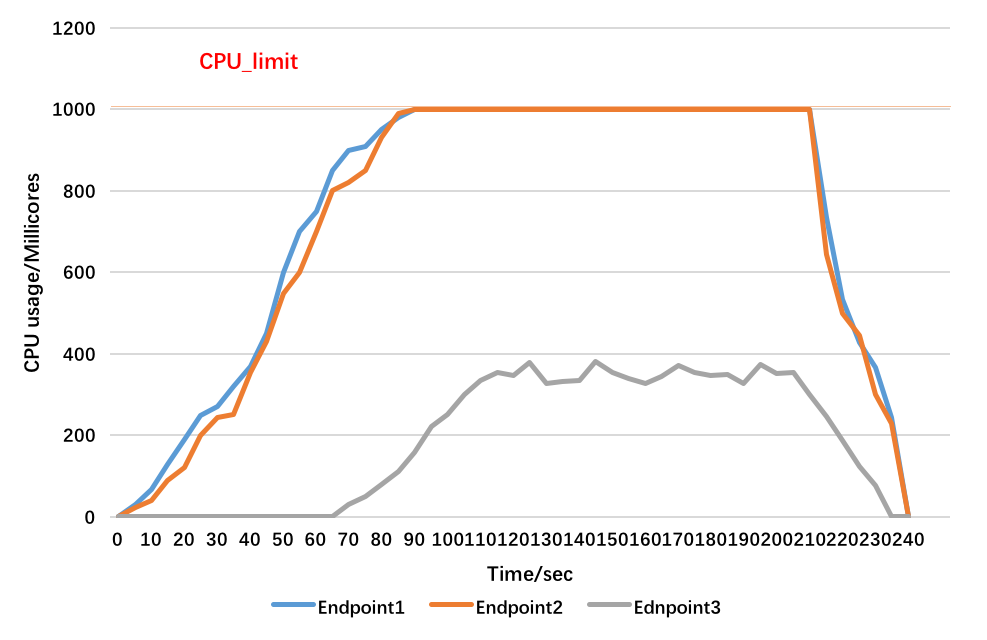
\includegraphics[width=0.45\textwidth]{images/data3.png}\\
 \caption{original controller under scaling pattern}
 \label{fig:original_scaling}
\end{figure}

\begin{figure}[!htb]
 \centering
 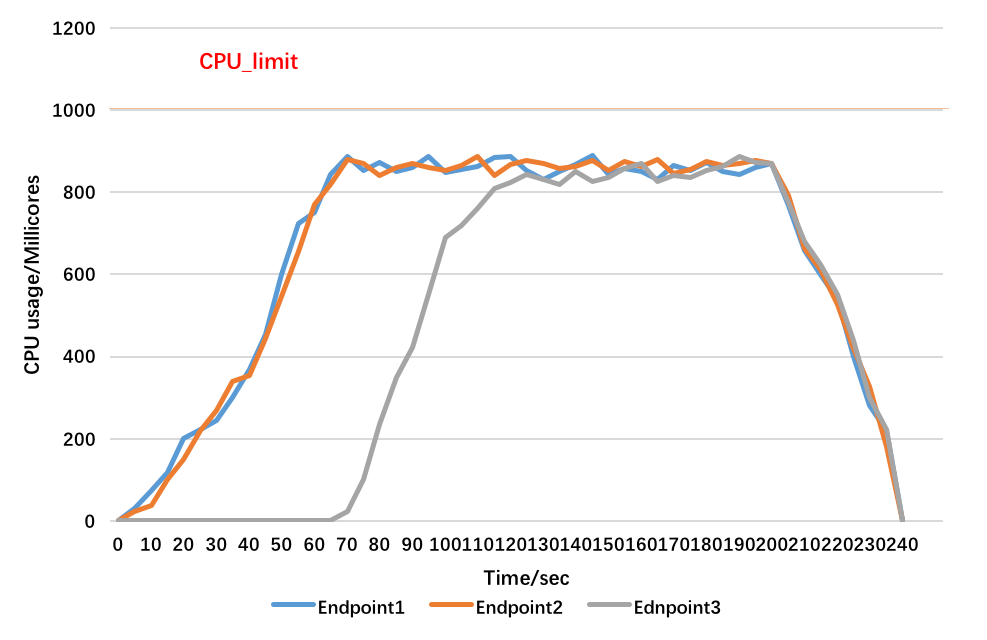
\includegraphics[width=0.45\textwidth]{images/data4.png}\\
 \caption{modified controller under scaling pattern}
 \label{fig:modified_scaling}
\end{figure}
Scaling pattern happens when administrator decides to scale up test applications because the workload is too large for current number of endpoint to handle. To emulate this pattern, we first deploy endpoint1 in node3 and endpoint2 in node3 and generate high workload to keep these two endpoints in high-loaded state but not overload. Then we deploy endpoint3 in node5 and increase the workload to the level that can keep three endpoints in high-loaded state ideally. Figure~{\ref{fig:original_scaling}} presents the performance of original ingress controller under scaling pattern and figure~{\ref{fig:modified_scaling}} shows the performance of modified ingress controller. Result shows that that when we increse workload at 65s, original ingress controller failes to dispatch appropriate workload to endpoint3, which should be assigned more workload to help endpoint1 and endpoint2. On the contrary, the modified ingress controller succeeds to lead more workload to endpint3, as a result, no endpoint becomes overhead. Table~{\ref{table:request_summary2}} points out that original ingress finishes 5844 requests, with 2956 503-request while the modified ingress controller finishes 8800 request with no 503-request, and the total number of reqeust is xxx.
\hspace{0pt}
\begin{table}[htbp]
 \begin{center}
  \begin{tabular}{c|c|c|c}
   \hline
            & Finished & 503  & Total \\  \hline
   Original & 5844     & 2956 & 8800  \\ \hline
   Modified & 8800     & 0    & 8800  \\ \hline
  \end{tabular}
 \end{center}
 \caption{Request summary of scaling pattern}
 \label{table:request_summary2}
\end{table}

Node-blocking pattern is established to evaluate performance of ingress controllers when their hosts are in high-loaded state. Firstly, we deploy endpoint1 in node3 and endpoint2 in node4. Then we generate workload for node3 to keep it on high-load state, leaving only enough resource for endpoint1. After that, we generate high workload to keep these two endpoints in high-loaded state but not overload and by comparing the RPS, we obtain performing disparity between original ingress controller and modified ingress controller. Through the comparison between figure~{\ref{fig:original_blocking}} and figure~{\ref{fig:modified_blocking}}, we find that it costs the original one about 260 second to handler 10000 requests while it costs the modified one only 250 seconds, which demonstrates the fact that load of host can affect the performance of endpoints. That is because the default isolation mechanism of docker, which is the container engine of kubernetes, can not support node-blocking pattern well. Kubernetes provides ${resource.request}$ and ${resource.limit}$ for users to allocate resource for their applications, however it does not gurantee the monopolization of resource. For example, the request limit and request of cpu are implemented by a combination of ${cgroup}$ commands: ${cfs\_quota\_us}$,${cfs\_period\_us}$ and ${cpushare}$. These commands insulates cpu through restricting the length of cpu time slice without binding applications to specific cpus, so when preemption happens, the inevitable context switch brings extra overhead. The modified ingress controller reduce context switch by taking load of host into consideration when balancing load so it gets a higher RPS.


\begin{figure}[!htb]
 \centering
 \includegraphics[width=0.45\textwidth]{images/data5.png}\\
 \caption{original controller under node-blocking pattern}
 \label{fig:original_blocking}
\end{figure}

\begin{figure}[!htb]
 \centering
 \includegraphics[width=0.45\textwidth]{images/data6.png}\\
 \caption{modified controller under node-blocking pattern}
 \label{fig:modified_blocking}
\end{figure}

Interrelationship pattern describes situation when several endpoints are deployed in the same node, we set up this pattern to figure out the ability of ingress controller to eliminate interrelationship between these endpoints. To emulate this pattern, we put endpoint1, endpoint2 in node3, and endpoint3  in node4. Then we generate high workload to keep these endpoints in high-loaded state. Figure~{\ref{fig:original_interrelationship}} shows that in original case, loads of endpoint1, endpoint2 are higher than other endpoints at the same time, and finally it finishes all requests in 245 seconds. That is because endpoints of the same application share the same resource feature, so if endpoints are deployed into the same node, their race for resource becomes fierce, thus they impact on performance of each other. Figure~{\ref{}} demonstrates that the modified ingress controller succeeds to reduce race and finishes all requests in 240 seconds.

\begin{figure}[!htb]
 \centering
 \includegraphics[width=0.45\textwidth]{images/data7.png}\\
 \caption{original controller under interrelationship pattern}
 \label{fig:original_interrelationship}
\end{figure}

\begin{figure}[!htb]
 \centering
 \includegraphics[width=0.45\textwidth]{images/data8.png}\\
 \caption{modified controller under interrelationship pattern}
 \label{fig:modified_interrelationship}
\end{figure}

Database-blocking pattern aims to figure out whether ingress controller can perform well under the micro service background. Under this circumstance, web applications tend to rely on each other rather than finish jobs independently, so QOS is not only decided by application itself, but also other applications it relies on. For convenience, we choose database-accessing applications as study case and set up database-blocking pattern: First we deploy endpoint1 in node3, endpoint2 in node4, endpoint3 in node5, database1 and database2 in node6, then we configure endpoint1, endpoint2 to connect to database1 and endpoint3 to database2. Finally, we generate workload to keep these endpoints in high-loaded state but not overhead. By comparing RPS, we get their performing disparity. Figure~{\ref{fig:original_database}} shows that original ingress controller failes to divide load of database1 to datebase2 which comes from endpoint1 and endpoint2. As a result, database1 bears more load than database2 all the time, pulling down the entire RPS. As figure~{\ref{fig:modified_database}} shown, modified ingress controller succeeds to balance load across database1 and database2, finishing all requests in 240 seconds.

\begin{figure}[!htb]
 \centering
 \includegraphics[width=0.45\textwidth]{images/data9.png}\\
 \caption{original controller under node-blocking pattern}
 \label{fig:original_database}
\end{figure}

\begin{figure}[!htb]
 \centering
 \includegraphics[width=0.45\textwidth]{images/data10.png}\\
 \caption{modified controller under node-blocking pattern}
 \label{fig:modified_database}
\end{figure}
